% Timing galaxy cluster mergers from radio and X-ray images
% Working draft skeleton. MNRAS template chosen for now; switching to AASTeX
% or A&A later is mostly a matter of the class file and the bibliography style.
%
% Build:  latexmk -pdf main.tex      (needs mnras.cls / mnras.bst, see README.md)
%
% Convention in this draft:
%   \todo{...}     things to write or decide
%   \stale{...}    figures or numbers that predate a fix and must be regenerated
%   bullet lists under each heading are talking points, not prose

\documentclass[fleqn,usenatbib]{mnras}

\usepackage[T1]{fontenc}
\usepackage{newtxtext,newtxmath}
\usepackage{graphicx}
\usepackage{amsmath}
\usepackage{xcolor}
\usepackage{booktabs}

\graphicspath{{figures/}}

\newcommand{\todo}[1]{\textcolor{red}{[TODO: #1]}}
\newcommand{\stale}[1]{\textcolor{orange}{[STALE: #1]}}
\newcommand{\tsc}{$t_{\rm sc}$}
\newcommand{\rfive}{$r_{500}$}
\newcommand{\mfive}{$M_{500}$}

% A figure slot for a plot we still need to make.
\newcommand{\figplaceholder}[2]{%
  \begin{figure}
    \centering
    \fbox{\parbox{0.9\columnwidth}{\centering\vspace{2em}
      \textbf{Figure to make}\\[0.5em]\small #1\vspace{2em}}}
    \caption{#2}
  \end{figure}}

\title[Merger timing from radio and X-ray images]{Timing galaxy cluster
mergers from radio and X-ray images with simulation-trained networks}

\author[J. Atkins et al.]{%
J. Atkins,$^{1}$\thanks{E-mail: \todo{email}}
C. Kong,$^{1}$
I. Dell'Antonio$^{1}$
\todo{full author list and order}
\\
$^{1}$\todo{affiliation}}

\date{Accepted XXX. Received YYY; in original form ZZZ}
\pubyear{2026}

\begin{document}
\label{firstpage}
\pagerange{\pageref{firstpage}--\pageref{lastpage}}
\maketitle

\begin{abstract}
\todo{Write last.} Talking points:
\begin{itemize}
  \item Merger timing (time since last collision) from images; TNG-Cluster
        (352 clusters), radio (DSA shock emission) and X-ray (Chandra mocks).
  \item Clean-image skill: pooled CNN $R^2 = 0.487 \pm 0.033$ (radio);
        X-ray $0.511$; joint $0.537$. Image adds $+0.083$ over scalar
        baselines and holds skill within mass bins.
  \item Physics: the model's radio emission is carried by cold, overdense,
        ram-pressure-stripped gas; a density cut fixes realism and accuracy.
  \item Forward modelling to LOFAR (field injection) and Chandra (real
        depths, backgrounds, redshift placement); realistic joint
        $R^2 \approx 0.44$.
  \item Applied to 25 LoVoCCS clusters; radio and X-ray predictions agree
        ($\rho = 0.62$); no ground truth, so framed as a demonstration.
\end{itemize}
\end{abstract}

\begin{keywords}
galaxies: clusters: general -- galaxies: clusters: intracluster medium --
radio continuum: general -- X-rays: galaxies: clusters -- methods: data
analysis -- methods: numerical
\end{keywords}

%======================================================================
\section{Introduction}
\label{sec:intro}
%======================================================================
\begin{itemize}
  \item Why merger timing matters: cluster assembly, particle acceleration,
        cosmology systematics (hydrostatic bias, mass calibration).
  \item Existing timing indicators and their limits: relic separation
        (Lee et al.\ 2024 relation in TNG-Cluster), X-ray morphology
        (centroid shift, concentration), galaxy phase space
        (arXiv:2509.20637 -- cannot tell past from future mergers, and
        explicitly suggests radio as the way to do so).
  \item ML on cluster images so far: mostly classification on idealised
        maps (Arendt et al.\ 2024, The300); representation learning on
        TNG-Cluster X-ray (ERGO-ML, Eisert et al.\ 2024). Few regress a
        timing variable; almost none carry the model to real data.
  \item Sim-to-real gap as the central problem: Bottrell et al.\ (2019)
        realism tiers; Ciprijanovic et al.\ (2021) domain adaptation.
  \item This paper: regression of time since collision from radio and
        X-ray images, a measured account of what the image adds beyond
        mass and brightness, and forward modelling to LOFAR and Chandra.
  \item \todo{State the contribution list crisply (4--5 items).}
\end{itemize}

%======================================================================
\section{Simulations and labels}
\label{sec:sims}
%======================================================================

\subsection{TNG-Cluster}
\begin{itemize}
  \item 352 zoom clusters, $M_{500} \sim 10^{14.0-15.3}\,{\rm M_\odot}$,
        snapshot 99 ($z = 0$); three orthogonal projections each.
  \item Halo-centred on \texttt{GroupPos}; note the earlier weight-centroid
        centring was off by a median 0.70\,\rfive\ (Appendix~\ref{app:audit}).
  \item \todo{Earlier full snapshots (91, 84) if included.}
\end{itemize}

\subsection{Radio emission model}
\begin{itemize}
  \item Hoeft \& Br\"uggen (2007) DSA emission per shocked cell
        (Mach $>1.3$, positive energy dissipation), as in Lee et al.\ (2024).
  \item Key finding: the emission is pathologically concentrated (one cell
        carries a median 29.5\% of a cluster's radio weight), and the cells
        that dominate are cold ($\sim$66\,000\,K), 379$\times$ overdense,
        Mach $\sim$26 gas at 1.37\,\rfive\ -- stripped ISM, not ICM.
  \item Density cut $n_{\rm H} < 10^{-4}\,{\rm cm^{-3}}$ on shock cells:
        improves realism against LoTSS and the CNN (paired $p = 0.010$).
        \todo{Pending Chuiyang's sign-off; justify physically.}
  \item Images: arcsinh-stretched projected weight, 128\,px over
        $\pm4$\,\rfive.
\end{itemize}
\figplaceholder{Emitting-gas phase diagram: temperature vs density of
shock cells, coloured by radio weight, before/after the density cut
(\texttt{check\_emitting\_gas.py} data).}{Where the radio weight sits.}

\subsection{X-ray mocks}
\begin{itemize}
  \item pyxsim APEC emission from hot, non-star-forming gas; soxs
        Chandra ACIS-I (Cycle 22) response, PSF, dither, particle
        background; originally 2\,Ms at $z = 0.05$.
  \item Field of view: only the ACIS-I square has data, $\pm$500\,kpc
        (0.3--0.6\,\rfive), \emph{not} $\pm1\,r_{500}$.
  \item Stretch: bare arcsinh is the identity at X-ray count rates; we use
        ${\rm arcsinh}(x/a)$ with one global $a$ (Section~\ref{sec:xray}).
\end{itemize}

\subsection{Merger-time labels}
\begin{itemize}
  \item Time since the most recent collision of \emph{any} mass ratio
        (merger catalogue of Lee et al.\ 2024; median ratio 1:11).
        \todo{Confirm definition with Chuiyang.}
  \item Pseudo-TSC (interpolated merger-score crossing) agrees at
        Spearman 0.961; which one we headline, and why.
  \item Major-merger-only labels are far less predictable
        ($R^2$ 0.435 $\to$ 0.074): radio morphology reflects recent
        disturbance of any size.
\end{itemize}
\figplaceholder{Label distribution: pseudo-TSC histogram and pseudo-TSC
vs merger-catalogue TSC scatter.}{The regression target.}

%======================================================================
\section{Observations}
\label{sec:obs}
%======================================================================
\begin{itemize}
  \item LoVoCCS sample; 25 targets with usable LoTSS DR3 cutouts
        (144\,MHz, 9$''$ beam), $z = 0.035$--$0.12$.
  \item AGN masking of compact sources (half-peak area vs beam).
  \item Chandra: 55 public observations of 19 targets; 15 ACIS-I targets
        processed (CIAO exposure maps, particle background from
        9.5--12\,keV, Cycle-22-equivalent exposure).
  \item Weak-lensing masses from LoVoCCS (single-peak NFW, M200c converted
        to M500c with the fit's own concentration); 17 of 25 targets.
  \item \todo{Table of targets: z, LoTSS rms, Chandra exposure/detector,
        $M_{\rm WL}$.}
\end{itemize}
\begin{figure*}
  \centering
  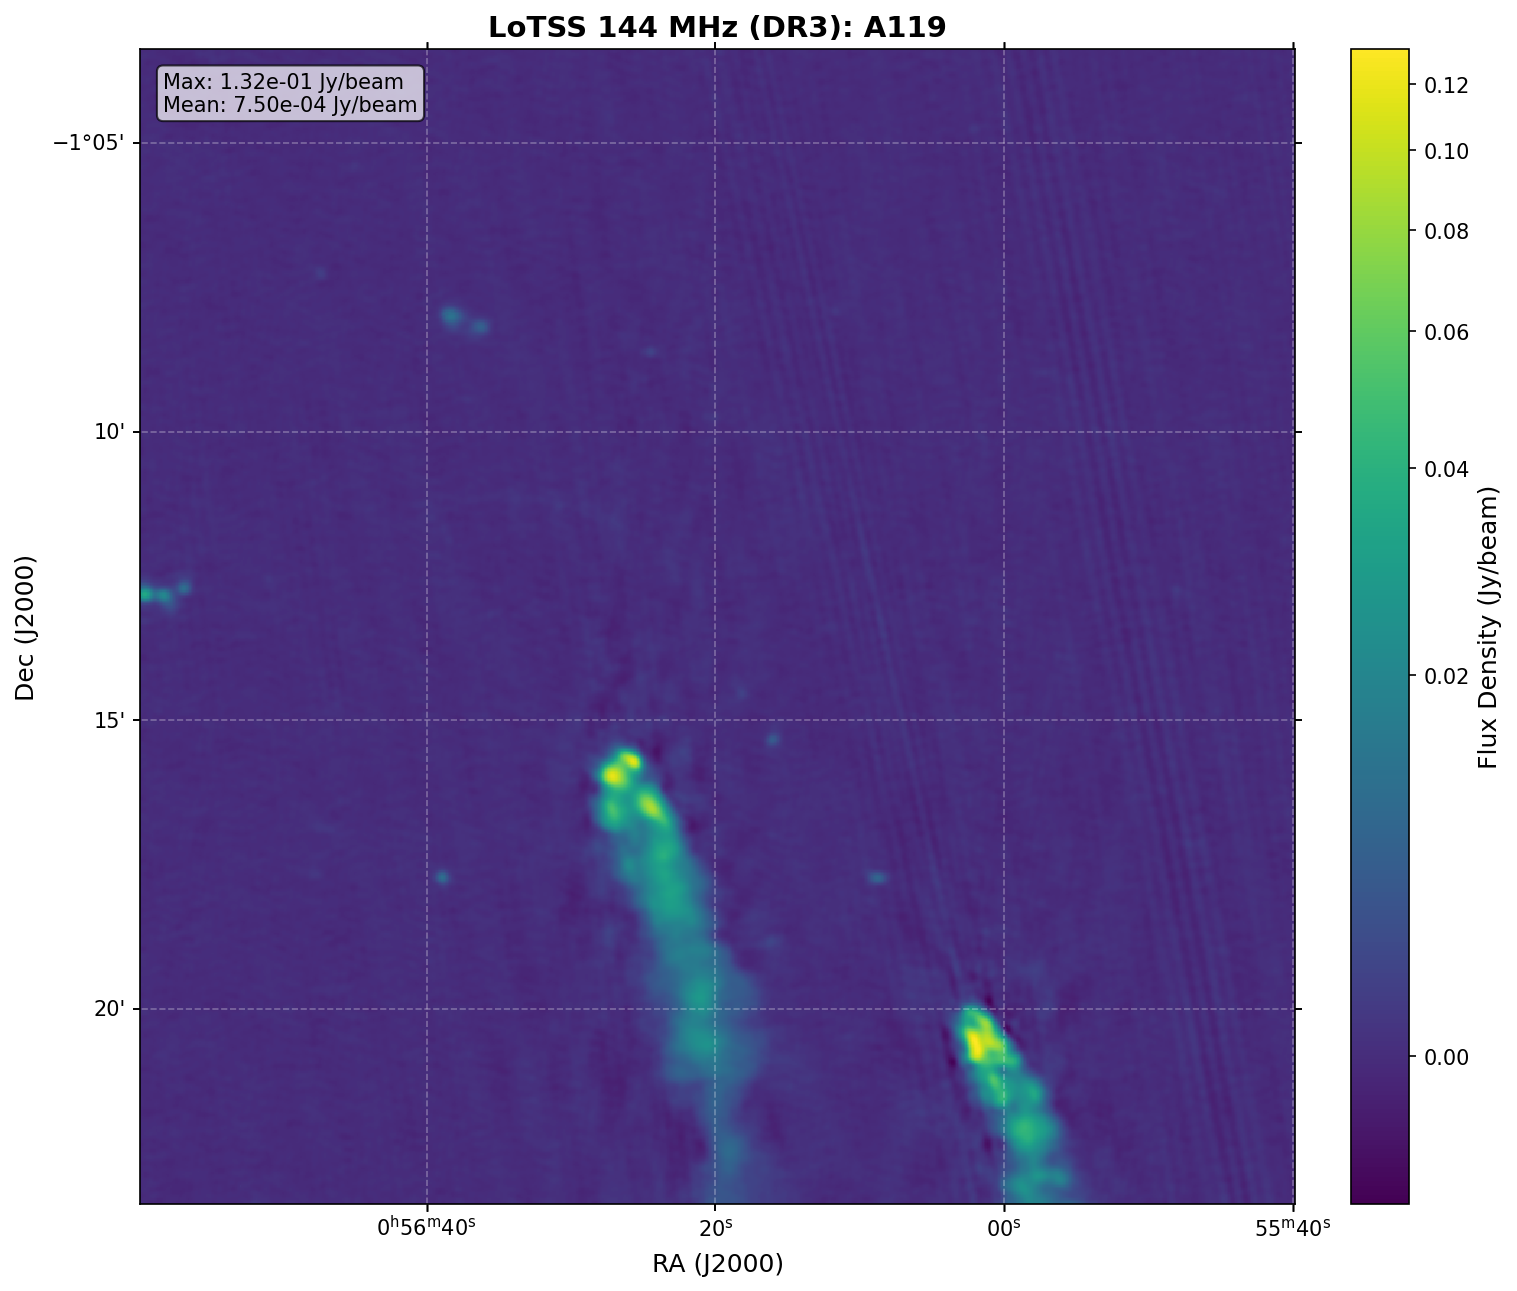
\includegraphics[width=0.48\textwidth]{lotss_A119.png}\hfill
  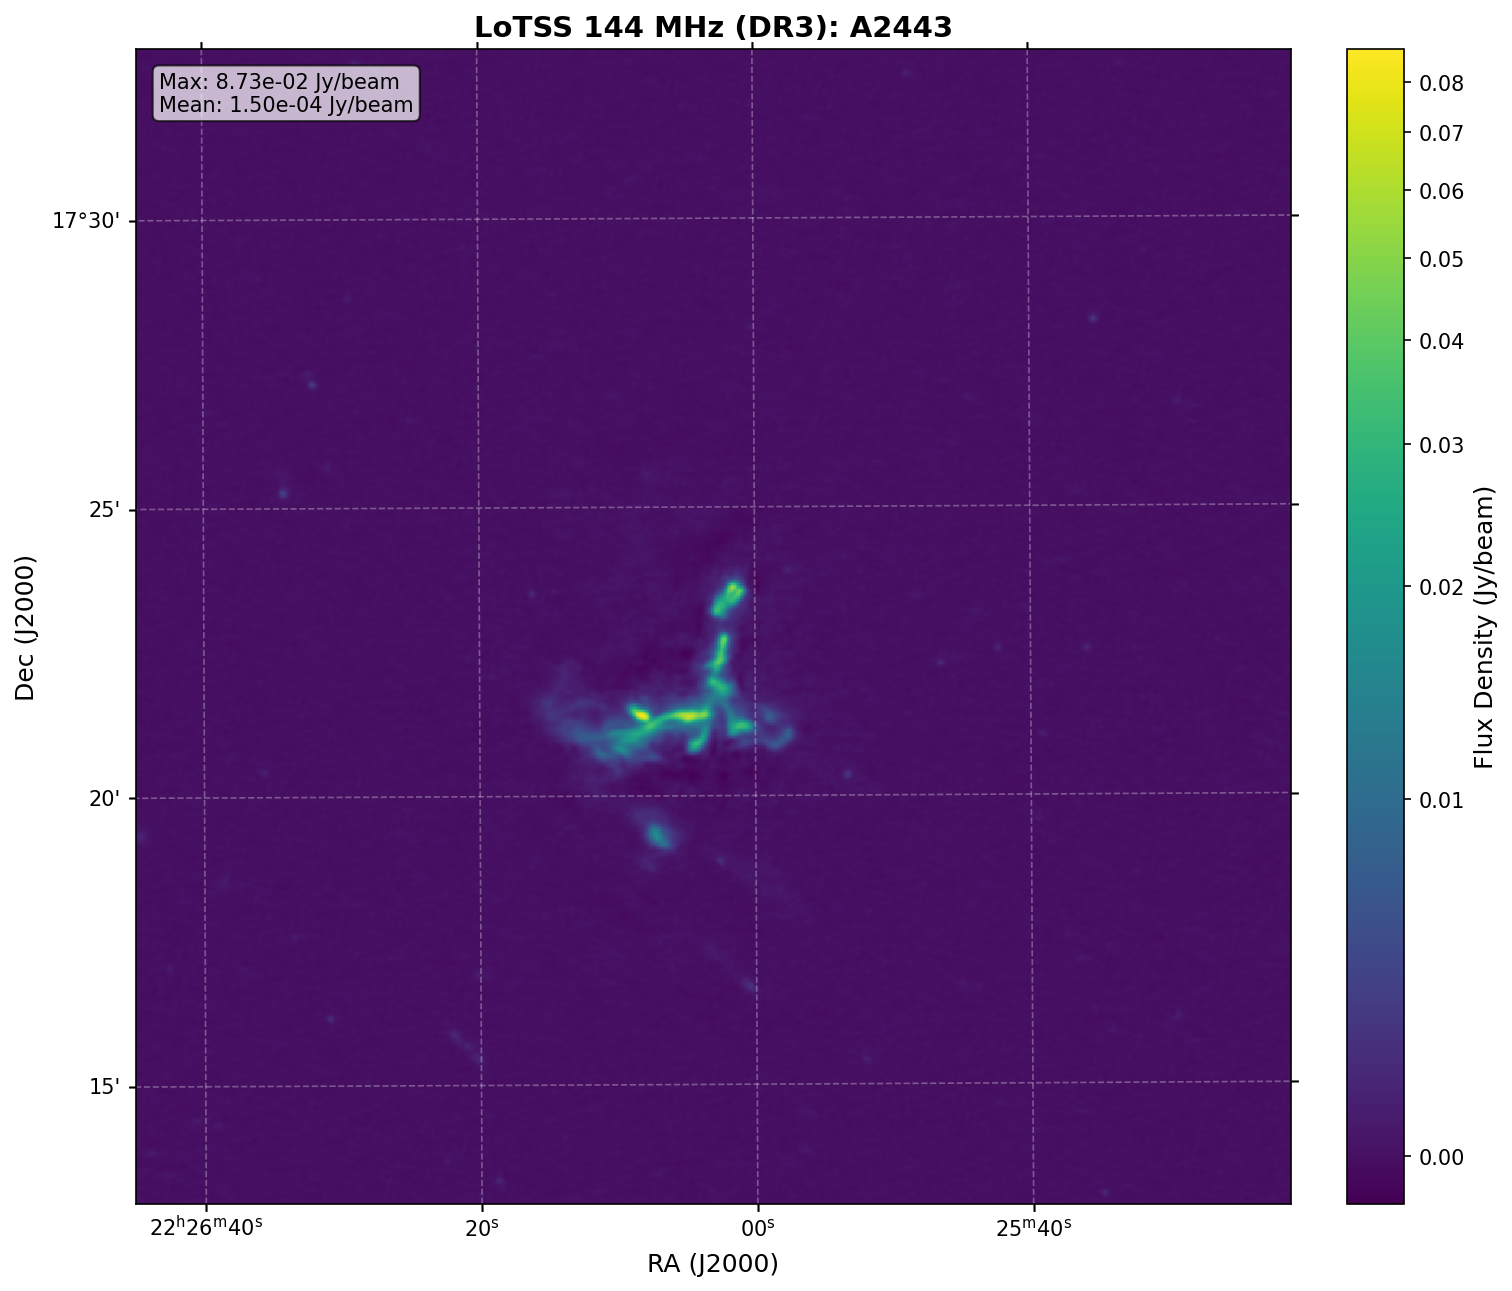
\includegraphics[width=0.48\textwidth]{lotss_A2443.png}
  \caption{Example LoTSS DR3 cutouts (A119, A2443).
  \todo{replace with a uniform gallery on the 1\,Mpc model grid, radio and
  Chandra side by side, for a handful of targets.}}
  \label{fig:obs_examples}
\end{figure*}

%======================================================================
\section{Forward modelling}
\label{sec:fwd}
%======================================================================

\subsection{Radio: from simulated maps to LoTSS}
\begin{itemize}
  \item Beam convolution, 1\,Mpc/128\,px common grid at each target's
        redshift.
  \item Noise must be beam-correlated: with white noise, real-cluster
        predictions ran to 10--27\,Gyr.
  \item Field injection into 208 real LoTSS DR3 fields (Bruno et al.\ 2023
        precedent; Bottrell ``FullReal'' tier): real noise, sources and
        artefacts.
  \item Flux: the simulation's own predicted power, one global constant
        -- \emph{not} an observed $P_{150}$--\mfive\ anchor
        (Section~\ref{sec:flux}).
  \item Realism: image statistics vs LoTSS as separations in mock
        standard deviations (KS $p$ values inflate with sample size).
\end{itemize}
\begin{figure*}
  \centering
  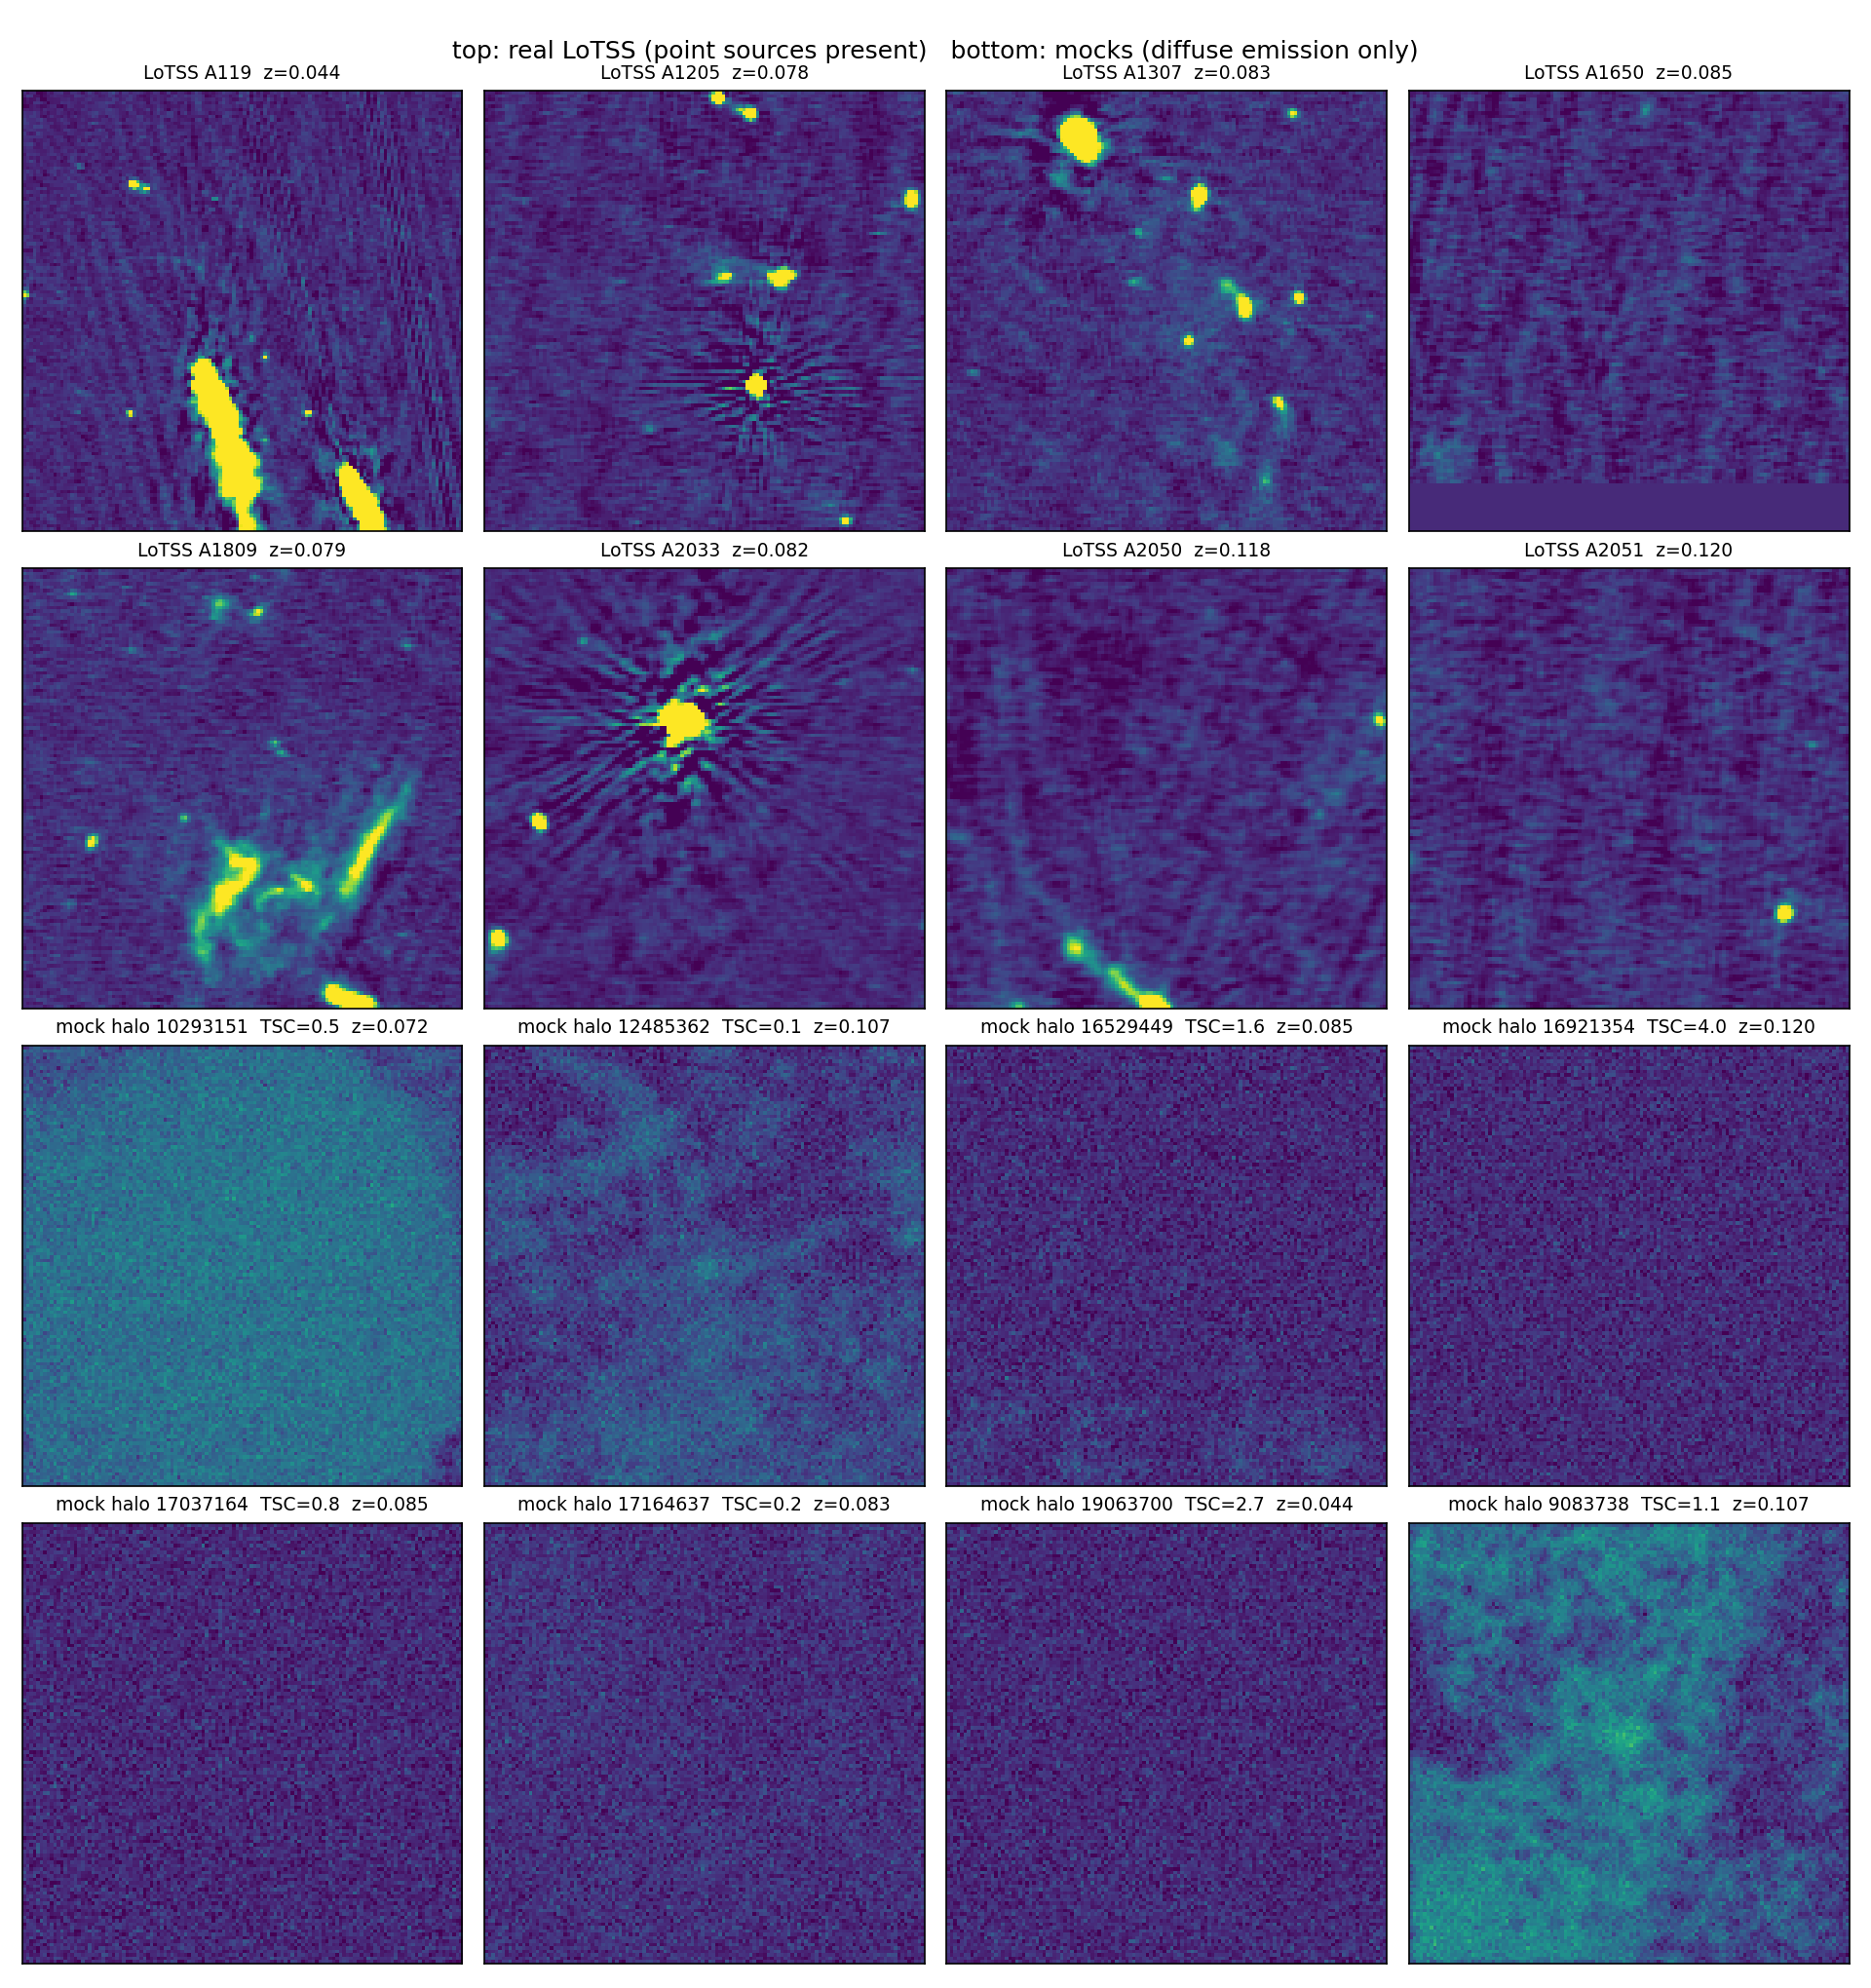
\includegraphics[width=\textwidth]{forward_examples.png}
  \caption{Simulated, forward-modelled and real LoTSS images.
  \stale{made before the noise-correlation fix and field injection;
  regenerate with \texttt{plot\_forward\_examples.py} on
  \texttt{injected\_nh4\_simflux.h5}.}}
  \label{fig:radio_gallery}
\end{figure*}

\begin{figure*}
  \centering
  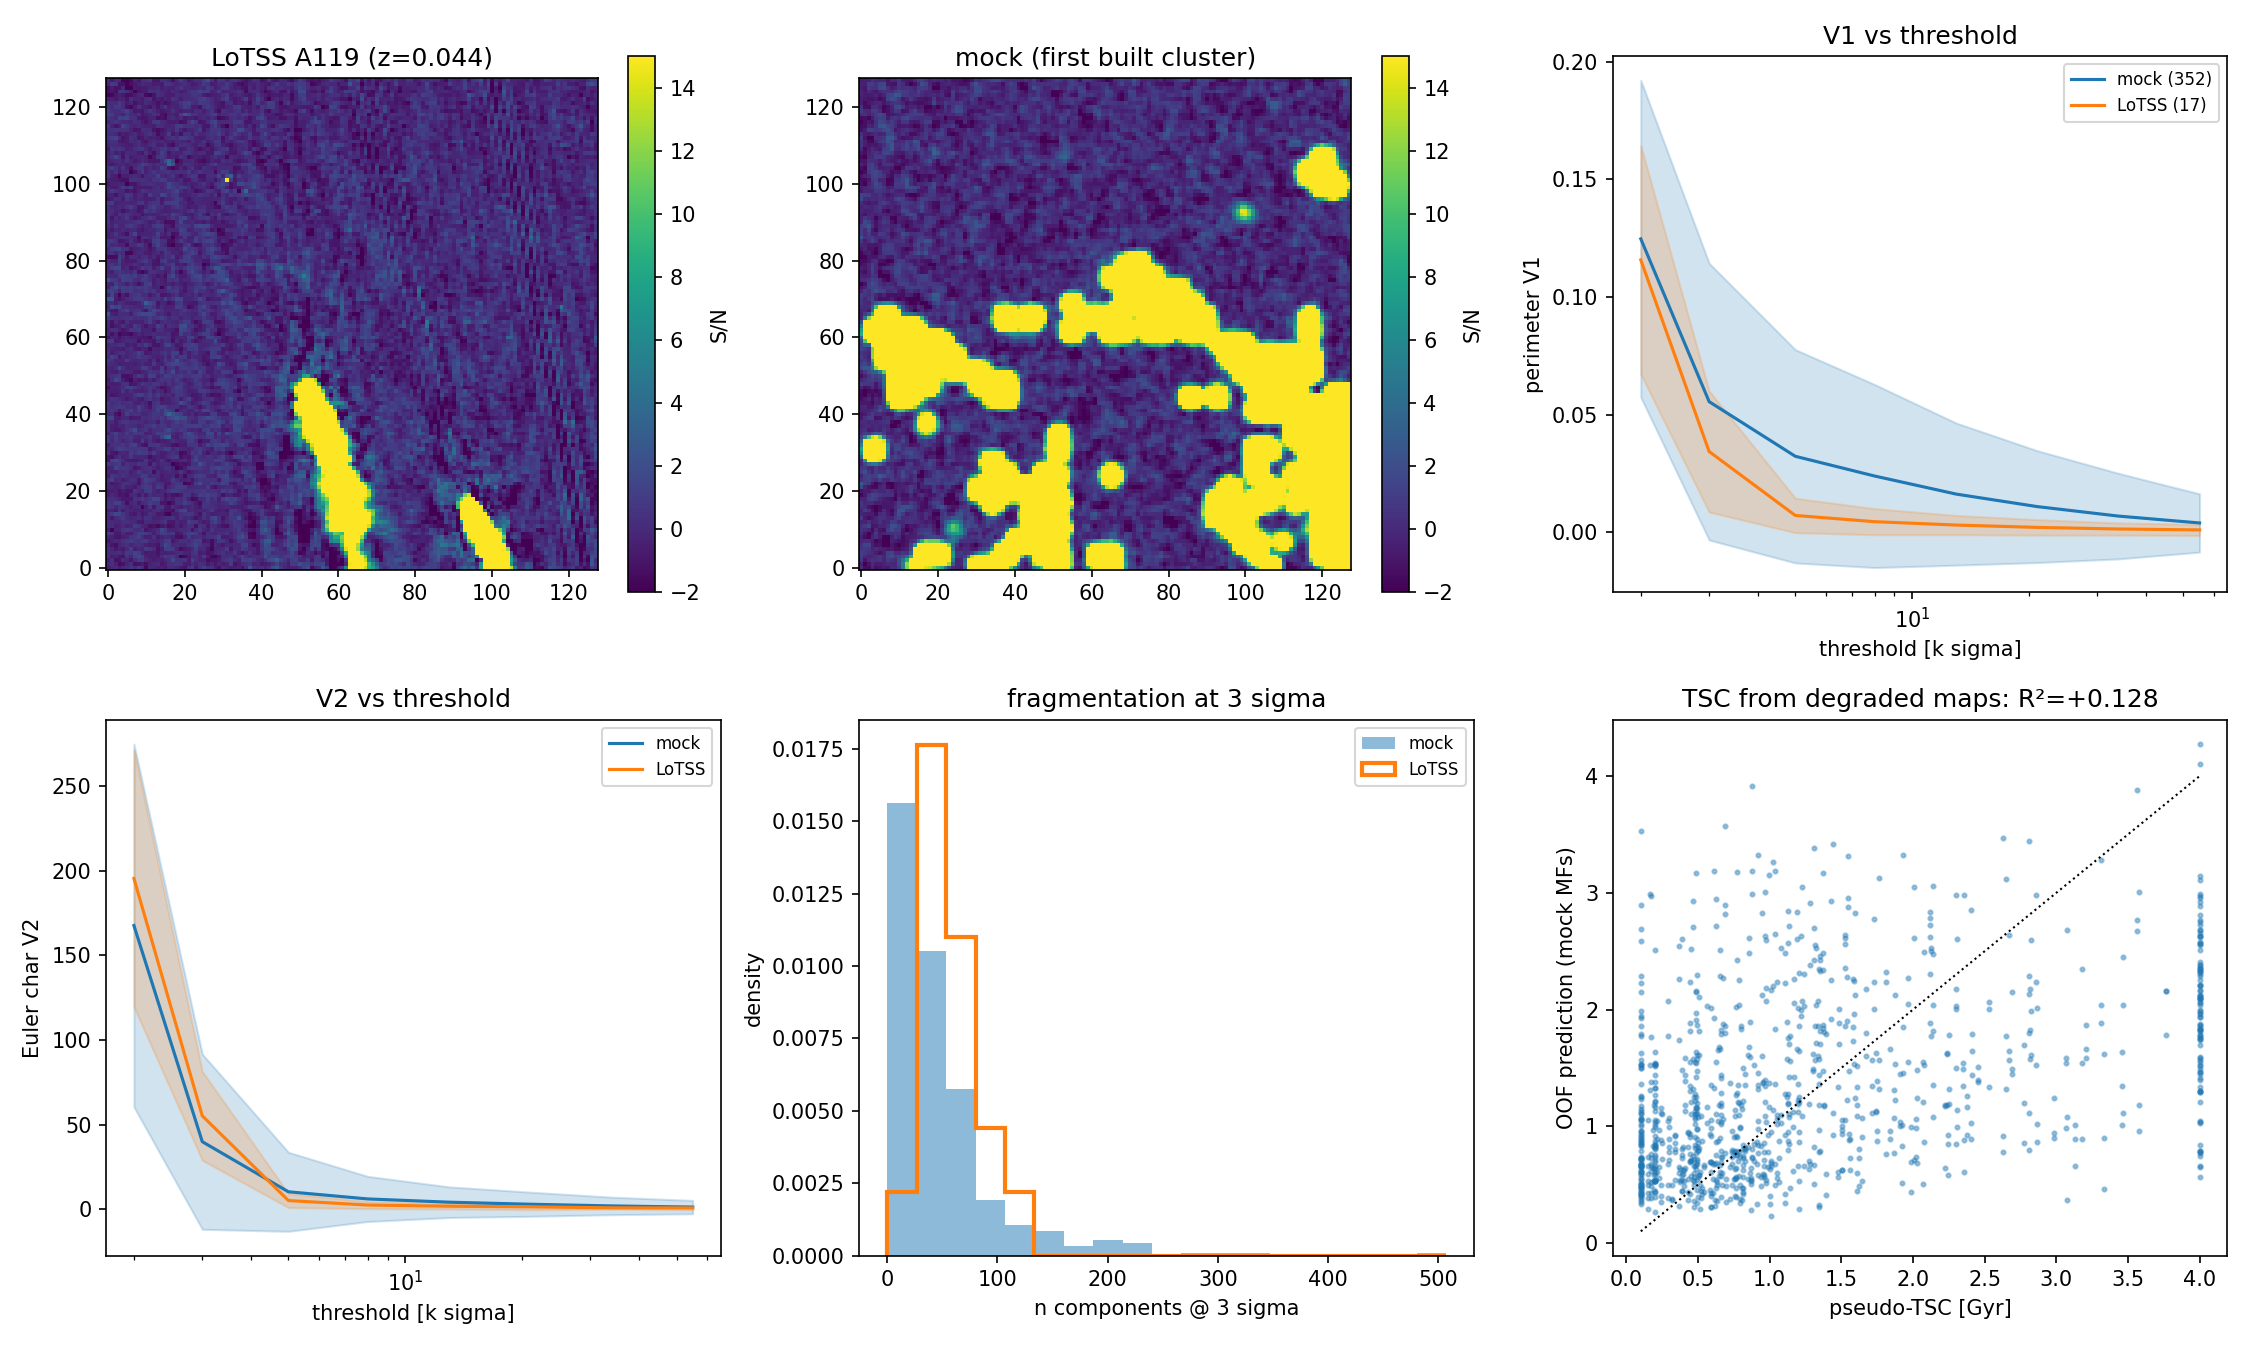
\includegraphics[width=\textwidth]{regen_nh4_arc_s0.png}
  \caption{Minkowski functionals of forward-modelled mocks against LoTSS:
  perimeter and Euler characteristic vs threshold, fragmentation at
  3$\sigma$, and merger time recovered from the mock functionals.
  \stale{analytic-noise tier with 17 targets, before field injection and
  the simulation-power flux; rerun on \texttt{injected\_nh4\_simflux.h5}
  with 25 targets, and quote separations rather than KS $p$ values.}}
  \label{fig:radio_mf}
\end{figure*}

\subsection{X-ray: from 2\,Ms mocks to real Chandra depths}
\label{sec:xray}
\begin{itemize}
  \item Binomial thinning of photon counts is an exact shallower
        observation; real archival depths (median 50\,ks all instruments,
        20\,ks ACIS-I).
  \item Sky backgrounds from soxs; particle background handled separately.
  \item Redshift placement: $1/D_L^2$ dimming, sky-area scaling of the
        background per (physically fixed) pixel, common aperture.
  \item TNG over-luminosity: mocks $\sim$3$\times$ brighter than real
        clusters (0.32 measured on Chandra; 0.28 from catalogue $L_X$);
        corrected with the catalogue value.
  \item Galactic absorption per target (small: median 2\%).
  \item Fig.~\ref{fig:lx}: the luminosity offset seen in catalogue $L_X$.
  \item Real-data processing and the particle-background normalisation
        lesson (effective-area-scaled exposure is wrong for unfocused
        background).
\end{itemize}
\begin{figure*}
  \centering
  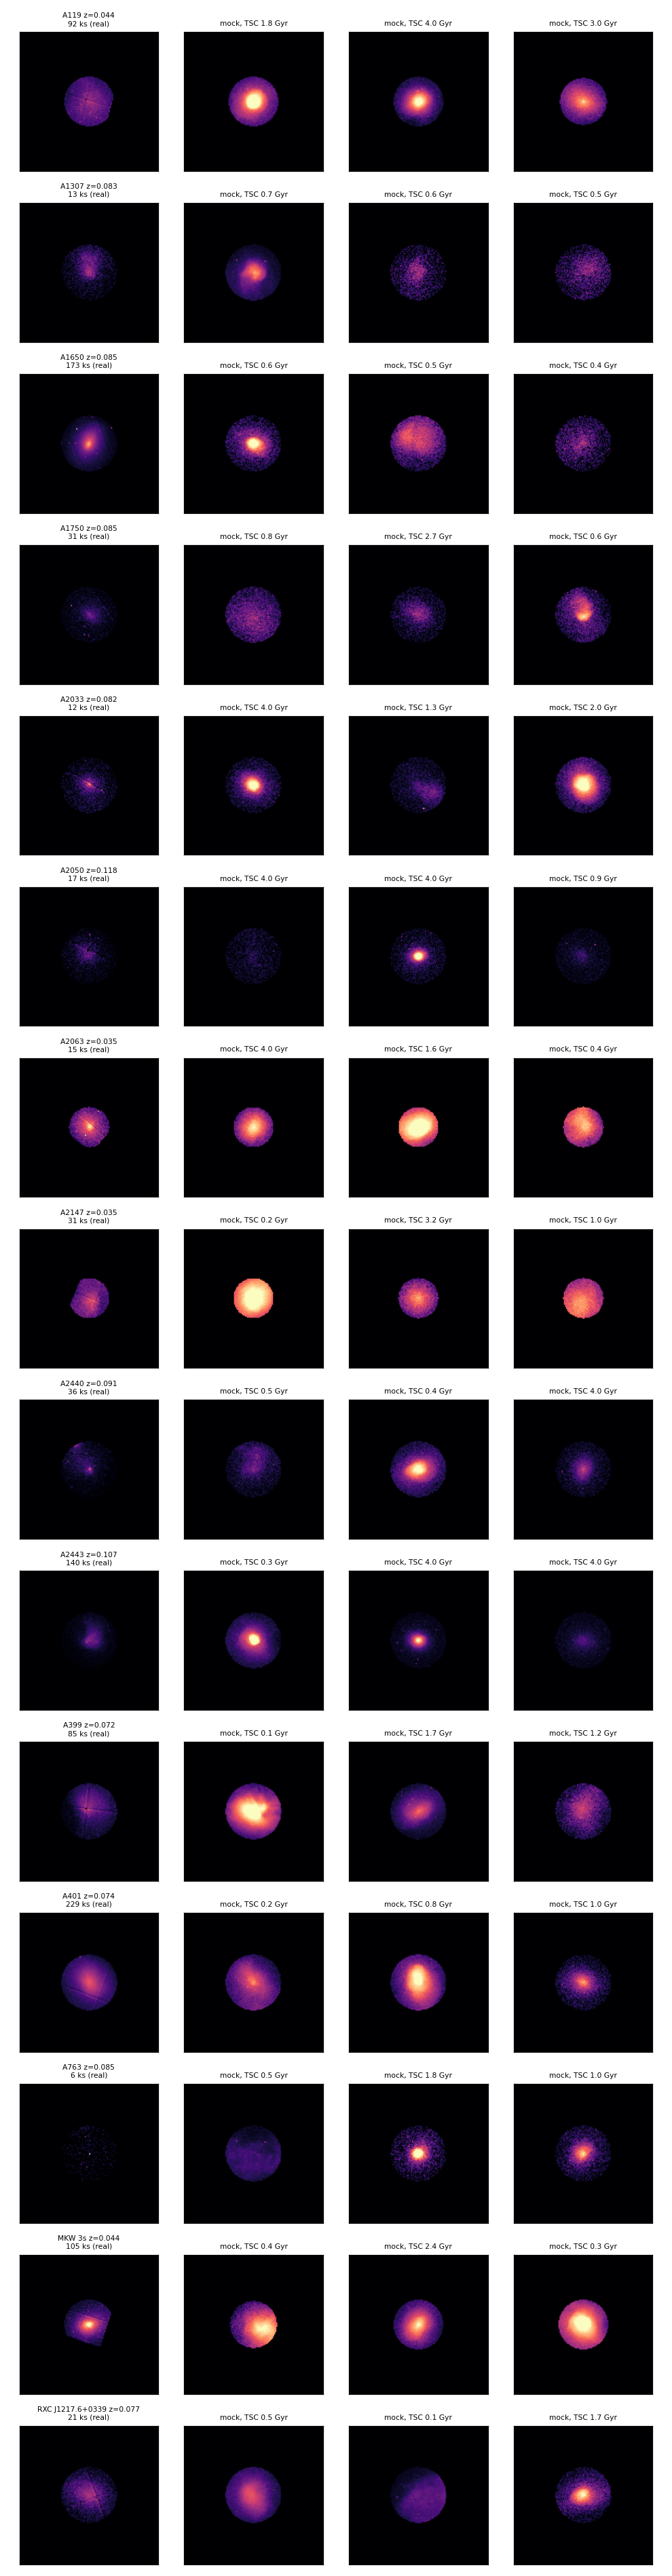
\includegraphics[width=0.7\textwidth]{xray_real_vs_mock.png}
  \caption{Real Chandra inputs (left column) beside redshift-matched mocks.
  \stale{made before the particle-background and sky-area fixes;
  regenerate with \texttt{plot\_xray\_real\_vs\_mock.py} on
  \texttt{xray\_real\_placed\_lx.h5}.}}
  \label{fig:xray_gallery}
\end{figure*}
\begin{figure*}
  \centering
  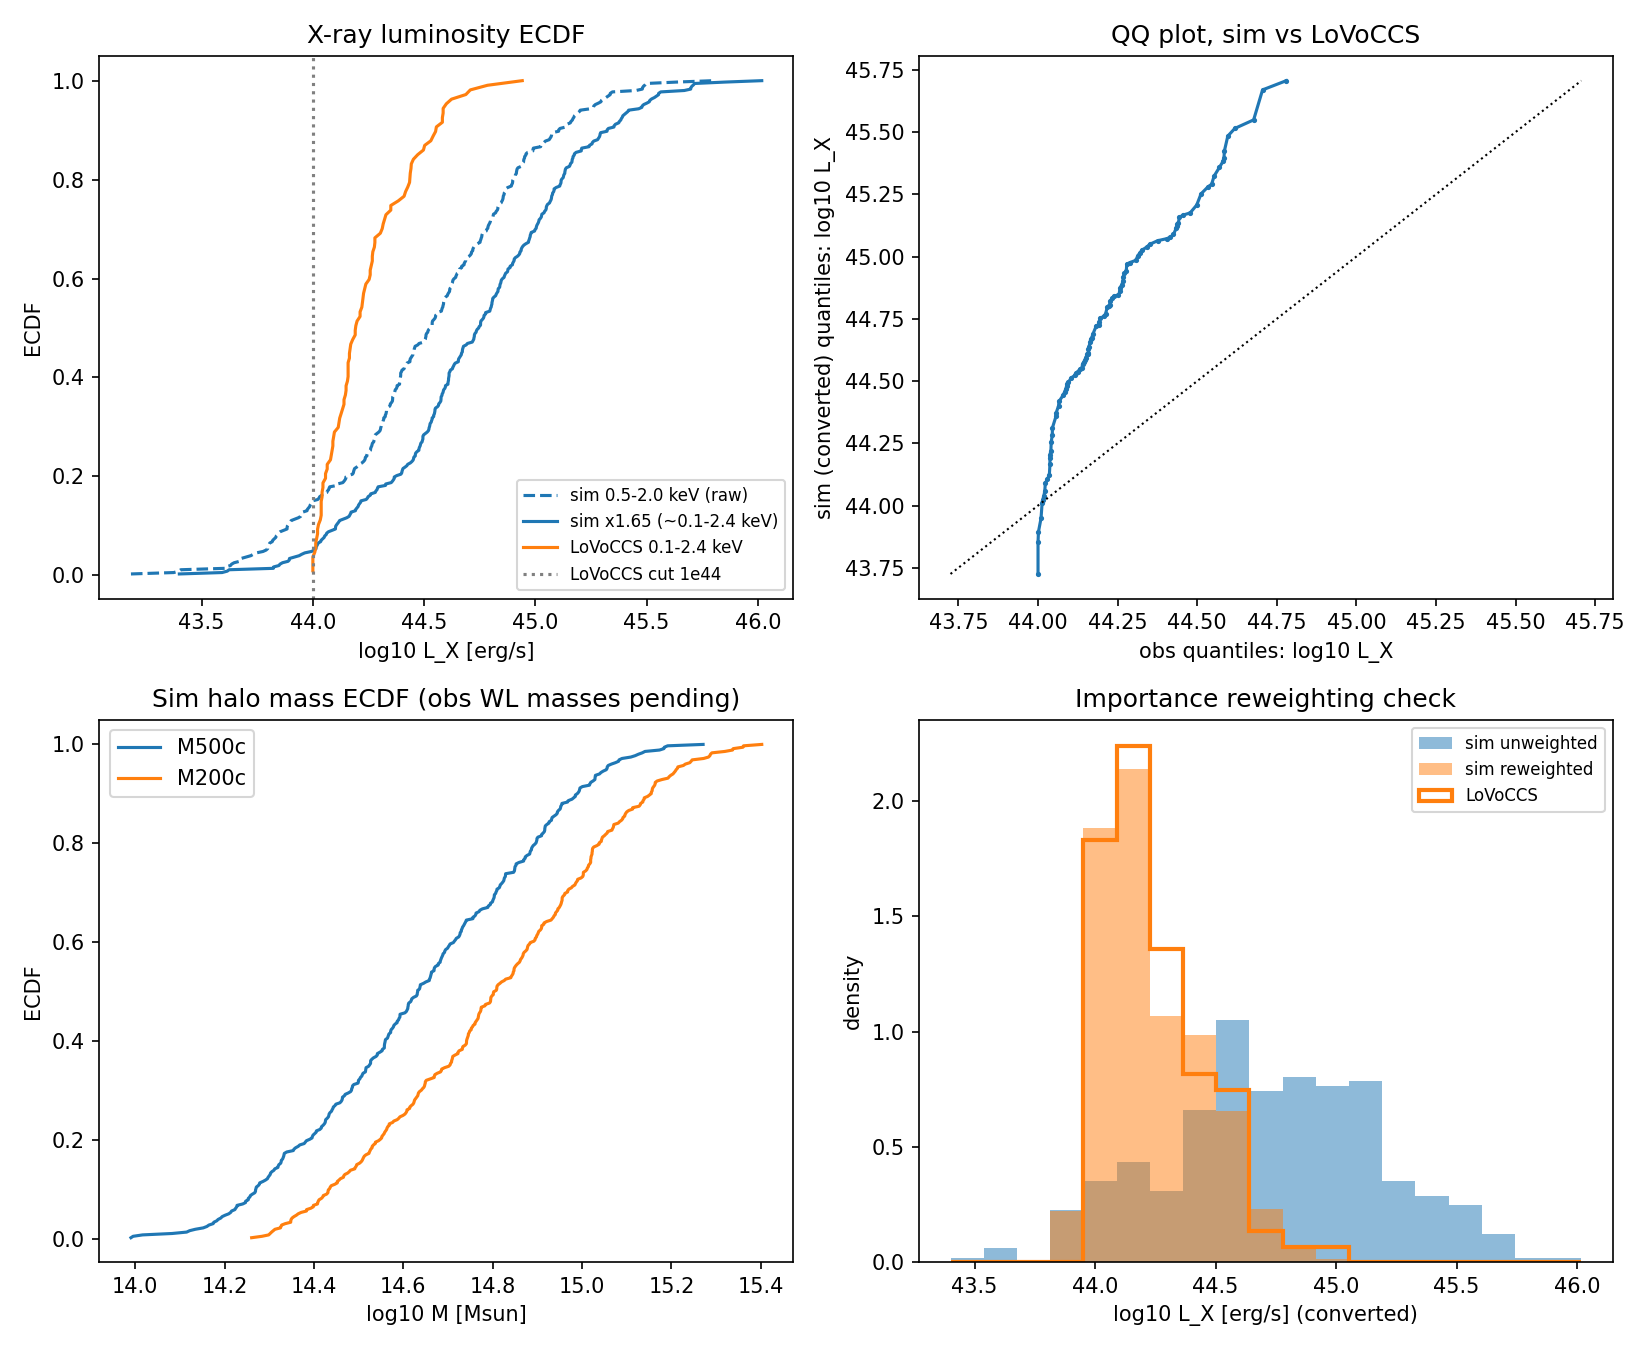
\includegraphics[width=0.8\textwidth]{sim_obs_dist.png}
  \caption{TNG-Cluster X-ray luminosities against the LoVoCCS sample:
  simulated clusters are $\sim$3.6$\times$ brighter at the same selection.
  \stale{the mass panel predates the weak-lensing masses; replace it with
  the mass-matched real/mock brightness comparison
  (\texttt{check\_xray\_domain\_gap.py}, median ratio 1.28 after
  correction). The reweighting panel belongs to a negative result.}}
  \label{fig:lx}
\end{figure*}
\figplaceholder{X-ray accuracy vs exposure (1\,ks to 2\,Ms) with the real
archive depth distribution overlaid (\texttt{summarize\_xray\_depth.py}).}
{X-ray skill survives realistic Chandra depths.}

%======================================================================
\section{Methods}
\label{sec:methods}
%======================================================================
\begin{itemize}
  \item Pooled CNN: shared encoder over three projections, mean-pooled;
        joint model with separate radio and X-ray encoders.
  \item Cross-validation: 5-fold, split by cluster; checkpoint chosen on an
        inner split of the training folds (selecting on the test fold
        inflated $R^2$ by 0.04--0.32; Appendix~\ref{app:audit}).
  \item Five seeds for headline numbers; paired tests across conditions.
  \item Baselines: halo mass, total flux, five-scalar ridge,
        Minkowski-functional XGBoost, X-ray morphology scalars.
  \item Mass conditioning: log\,\mfive\ as an input, blurred by the real
        weak-lensing errors.
\end{itemize}

%======================================================================
\section{Results}
\label{sec:results}
%======================================================================

\subsection{What the radio image knows}
\begin{itemize}
  \item Pooled CNN $0.487 \pm 0.033$ (ensemble 0.528) vs total flux 0.432,
        mass 0.314, five scalars 0.455.
  \item Within mass terciles: CNN 0.33/0.32/0.22 while scalars fall to
        $-0.28$ in the high-mass bin; partial $\rho = 0.475$ at fixed mass.
  \item Morphology alone (flux-normalised maps): 0.418; but shape and
        brightness are not separable (shape-only model 59\% predictable
        from the flux it never saw).
  \item Caveat: scalars explain 72\% of the CNN output.
  \item Minkowski functionals as an interpretable baseline: XGBoost on 48
        topology numbers reaches 0.454; fragmentation rises with merger age.
\end{itemize}
\begin{figure*}
  \centering
  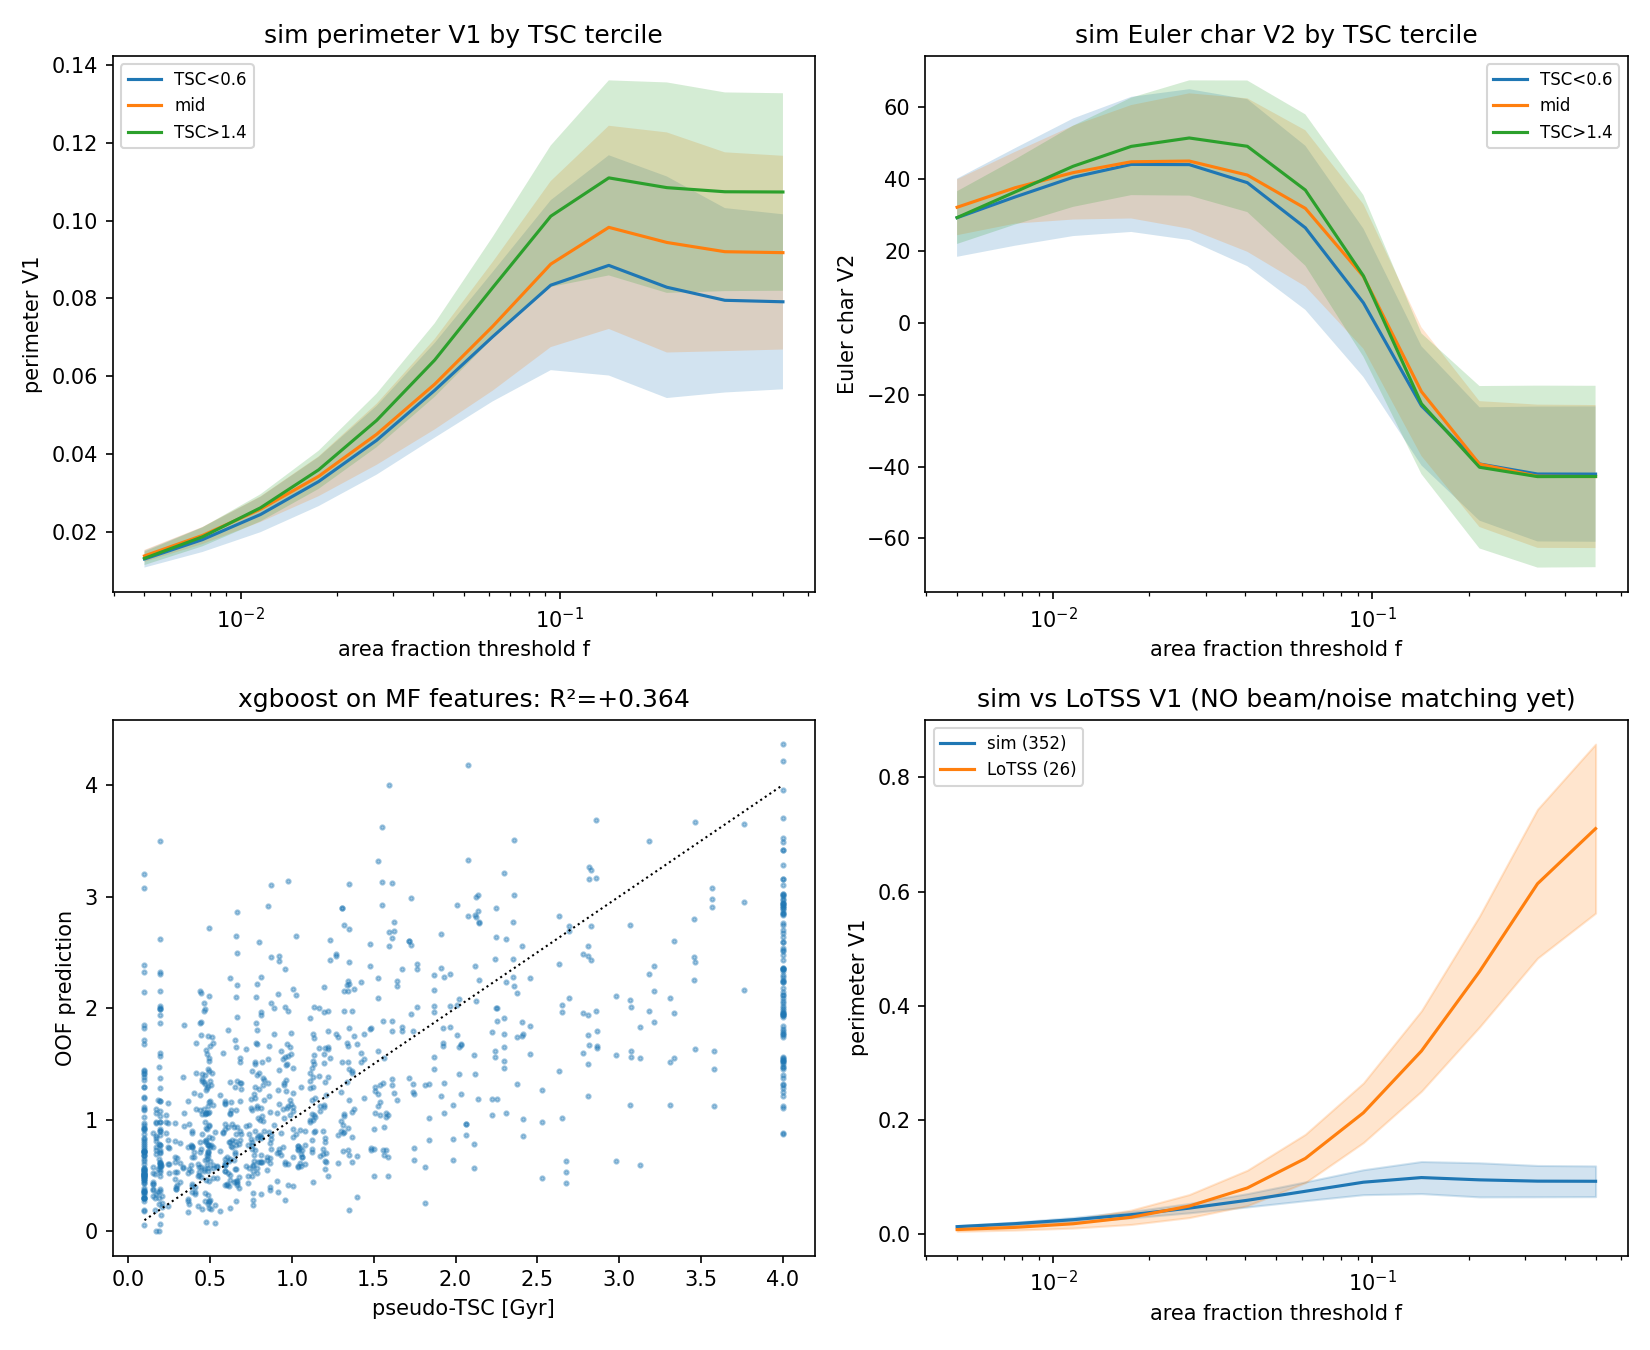
\includegraphics[width=\textwidth]{minkowski.png}
  \caption{Minkowski functionals of the simulated radio maps and their
  relation to merger time.
  \stale{built on weight-centroid-centred maps before the density cut and
  the protocol fix; rerun \texttt{minkowski\_functionals.py} on
  \texttt{dataset\_nh4\_128.h5}.}}
  \label{fig:mf}
\end{figure*}
\figplaceholder{Bar chart: OOF $R^2$ of the scalar baselines, morphology
only, CNN, ensemble (\texttt{analyze\_mass\_control.py},
\texttt{compare\_shape.py}).}{The image against scalar baselines.}
\figplaceholder{True vs predicted TSC, with residuals by age bin
(\texttt{plot\_tsc\_predictions.py} on saved OOF predictions).}
{Predicted against true merger time.}

\subsection{X-ray, and radio with X-ray}
\begin{itemize}
  \item The stretch bug and fix: X-ray 0.320 $\to$ 0.511 ($p = 0.0003$).
  \item Joint model $0.537 \pm 0.016$: beats radio by $+0.050$ and X-ray by
        $+0.026$; gains on older mergers (RMSE $>2$\,Gyr 1.25 $\to$ 1.13).
\end{itemize}

\subsection{Under observational degradation}
\label{sec:flux}
\begin{itemize}
  \item Anchored vs simulation-power flux: 0.338 $\to$ 0.412; image beyond
        mass $+0.079 \to +0.151$; $\rho({\rm pred}, M)$ $-0.89 \to -0.61$.
  \item The simulation's $P_{150}$--\mfive: slope $3.30\pm0.33$ (obs.\ 3.55),
        scatter 1.65\,dex (obs.\ 0.35); scatter tracks merger state with
        the observed sign.
  \item Realistic X-ray and joint (after all background fixes): X-ray 0.339,
        joint 0.438. \todo{5 seeds; snapshot 91.}
\end{itemize}
\figplaceholder{Simulated $P_{150}$--\mfive\ relation coloured by TSC,
with the Cuciti et al.\ (2023) fit (\texttt{summarize\_b23.py} data).}
{The simulation's own mass--power relation.}

\subsection{Application to LoVoCCS}
\begin{itemize}
  \item Predictions for 25 (radio), 15 (X-ray), 14 (joint) clusters; all
        within the label range.
  \item Radio and X-ray agree: $\rho = 0.62$ ($p = 0.019$), 0.67 at fixed
        $z$; at fixed weak-lensing mass 0.38 ($n = 10$, n.s.).
  \item A399/A401 youngest -- but mass-driven; do not present as
        validation.
  \item Weak-lensing peak check: only 9 overlapping clusters,
        inconclusive.
\end{itemize}
\figplaceholder{Radio vs X-ray predictions for the 14 clusters with both,
coloured by weak-lensing mass (\texttt{compare\_real\_preds.py}).}
{Two independent observables on real clusters.}

%======================================================================
\section{Discussion}
\label{sec:discussion}
%======================================================================
\begin{itemize}
  \item What sets the emission in the model, and what the density cut
        implies for simulated relic studies.
  \item Brightness vs morphology: the honest decomposition.
  \item Mocks too bright (X-ray) and too scattered (radio power): what that
        says about TNG-Cluster.
  \item Tension with the relic-separation relation. \todo{Reconcile after
        talking to Lee's group (sample selection).}
  \item Limitations: 352 clusters; no ground truth on real clusters;
        early-epoch Chandra soft background; image-plane (not uv-plane)
        radio injection; X-ray field of view.
  \item Negative results worth recording: synthetic diffusion
        augmentation, CAMELS, $L_X$ reweighting, relic-distance clocks,
        cell-volume deposition.
\end{itemize}

%======================================================================
\section{Conclusions}
\label{sec:conclusions}
%======================================================================
\todo{Numbered list of findings, written last.}

\section*{Acknowledgements}
\todo{TNG-Cluster, LOFAR/LoTSS, Chandra archive, LoVoCCS, computing
(Brown CCV).}

\section*{Data Availability}
\todo{Code repository, derived catalogues, predictions.}

\bibliographystyle{mnras}
\bibliography{refs}

\appendix

\section{Audit of the pipeline}
\label{app:audit}
\begin{itemize}
  \item Checkpoint selection on the test fold: $+0.043$ (baselines),
        $+0.32$ (mock transfer); fixed with inner-split selection.
  \item Weight-centroid centring (median 0.70\,\rfive\ off).
  \item Name-key and cutout-size bugs (17 $\to$ 25 real clusters).
  \item X-ray stretch; X-ray background normalisation; background sky-area
        scaling.
  \item \todo{Decide how much of this belongs in the paper vs the repo.}
\end{itemize}

\section{Negative results}
\label{app:negative}
\begin{figure}
  \centering
  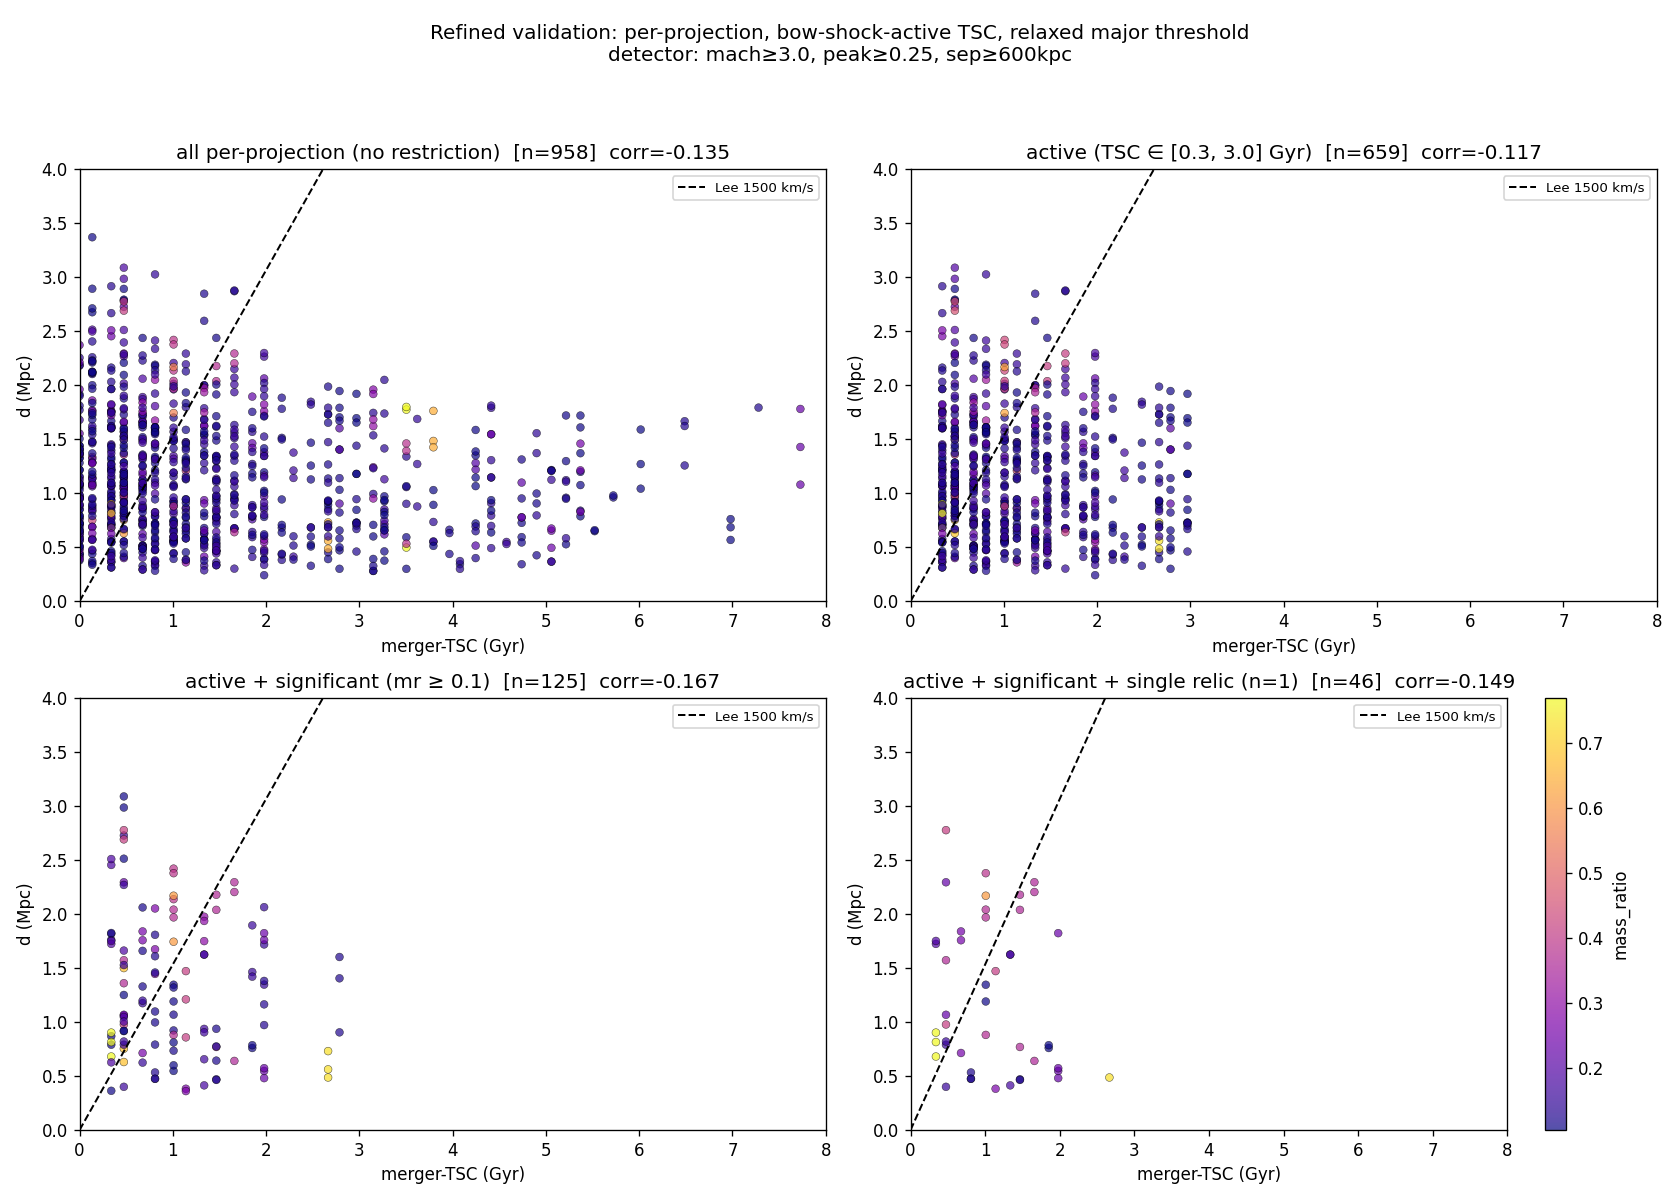
\includegraphics[width=\columnwidth]{relic_v3_validation.png}
  \caption{Relic separation against merger time in TNG-Cluster, four
  slicings: no positive relation.
  \stale{labels and centring predate the audit; re-check before use.}}
  \label{fig:relic_null}
\end{figure}

\begin{figure}
  \centering
  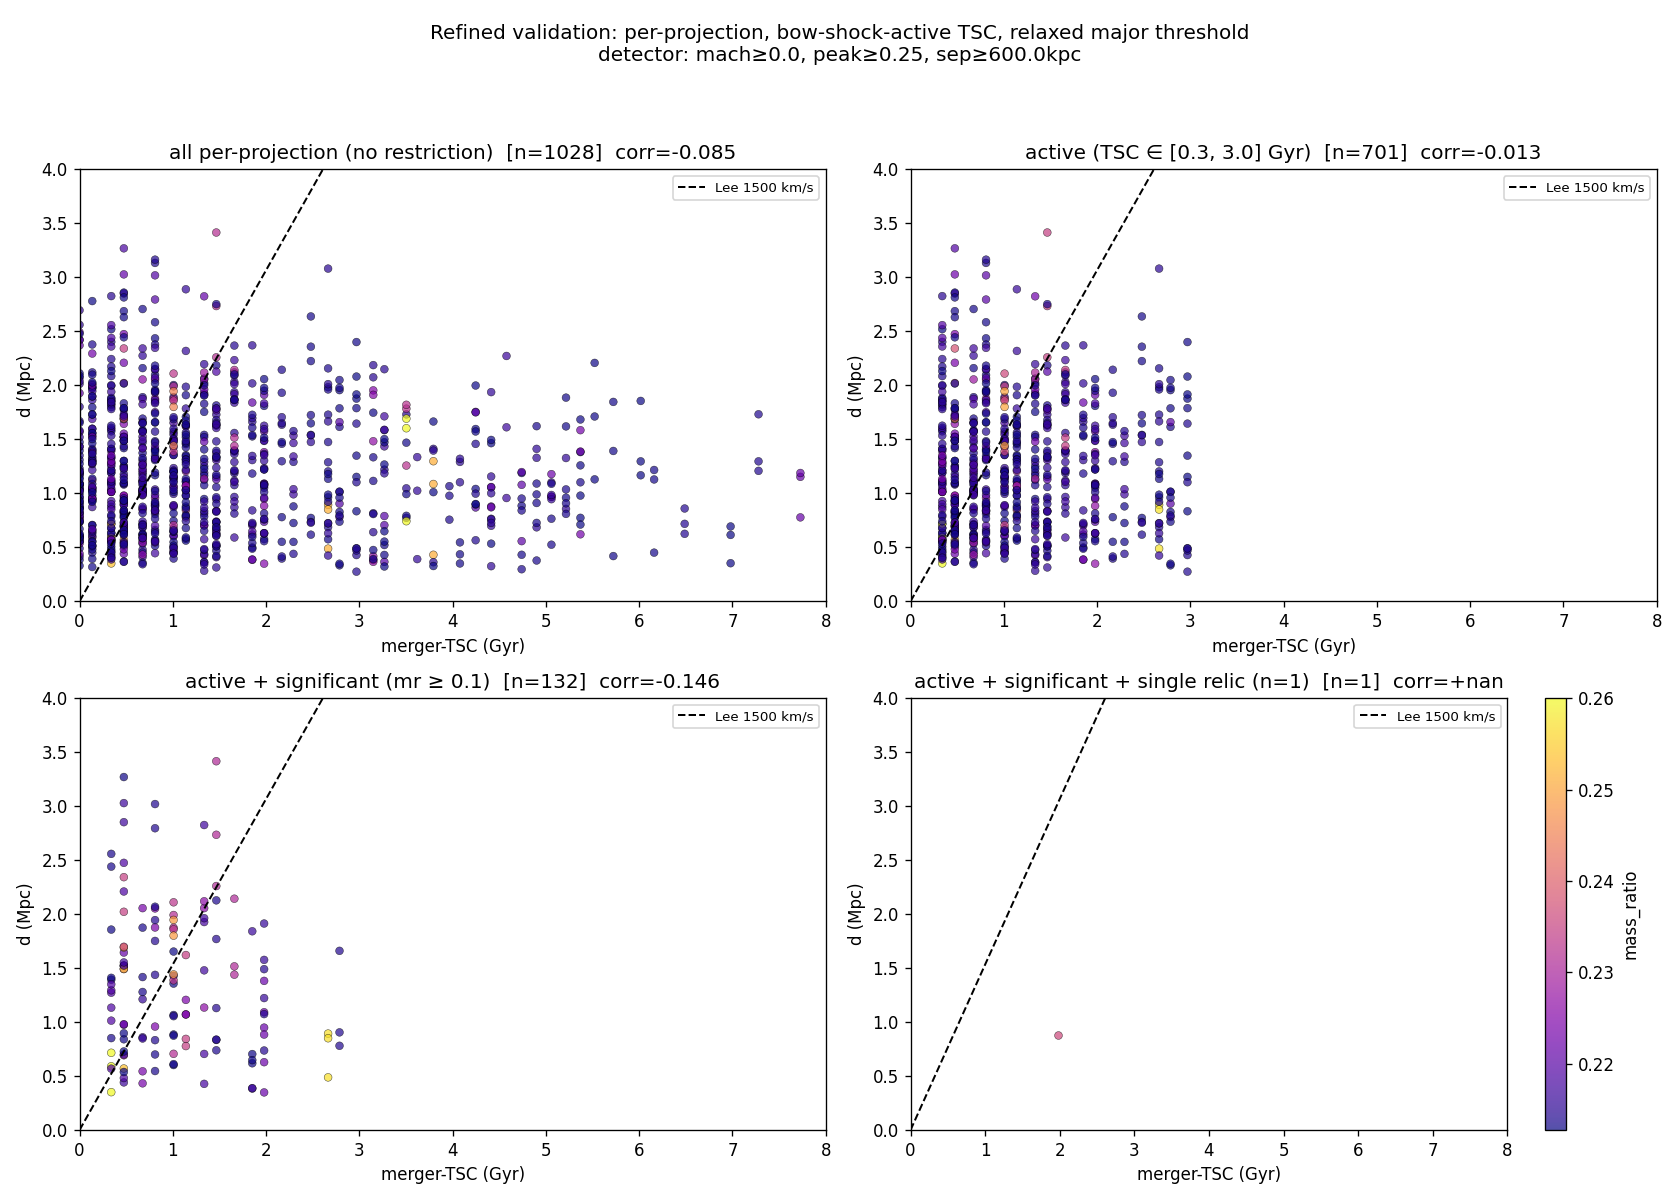
\includegraphics[width=\columnwidth]{relic_radio_validation.png}
  \caption{The same test with relics detected directly in the radio maps
  rather than from shock cells.
  \stale{predates the audit.}}
  \label{fig:relic_radio}
\end{figure}

\begin{figure}
  \centering
  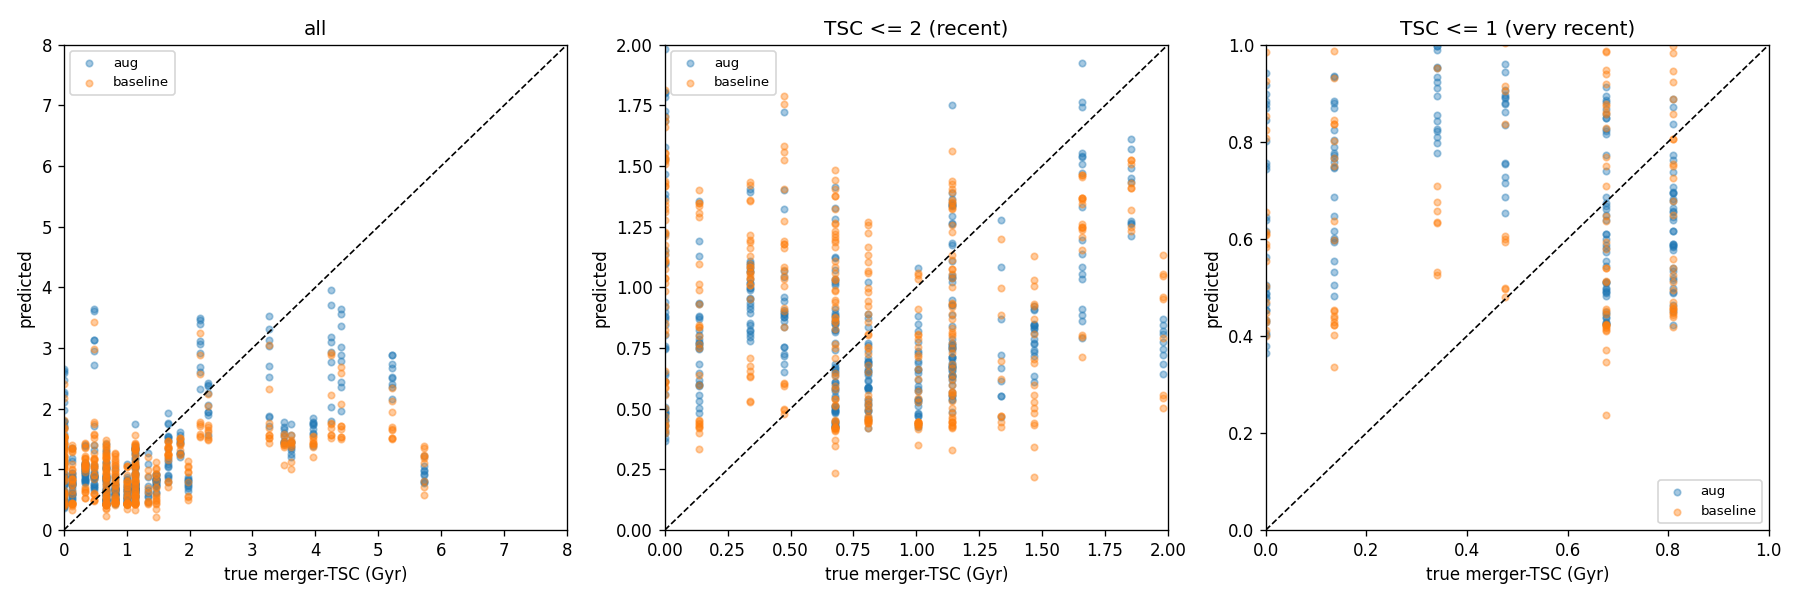
\includegraphics[width=\columnwidth]{aug_comparison_128.png}
  \caption{CNN with and without diffusion-generated augmentation: no gain
  under cross-validation.
  \stale{single-split protocol shown; the 5-fold result (no gain,
  $\Delta R^2 = +0.001$) needs its own plot.}}
  \label{fig:aug}
\end{figure}

\begin{figure}
  \centering
  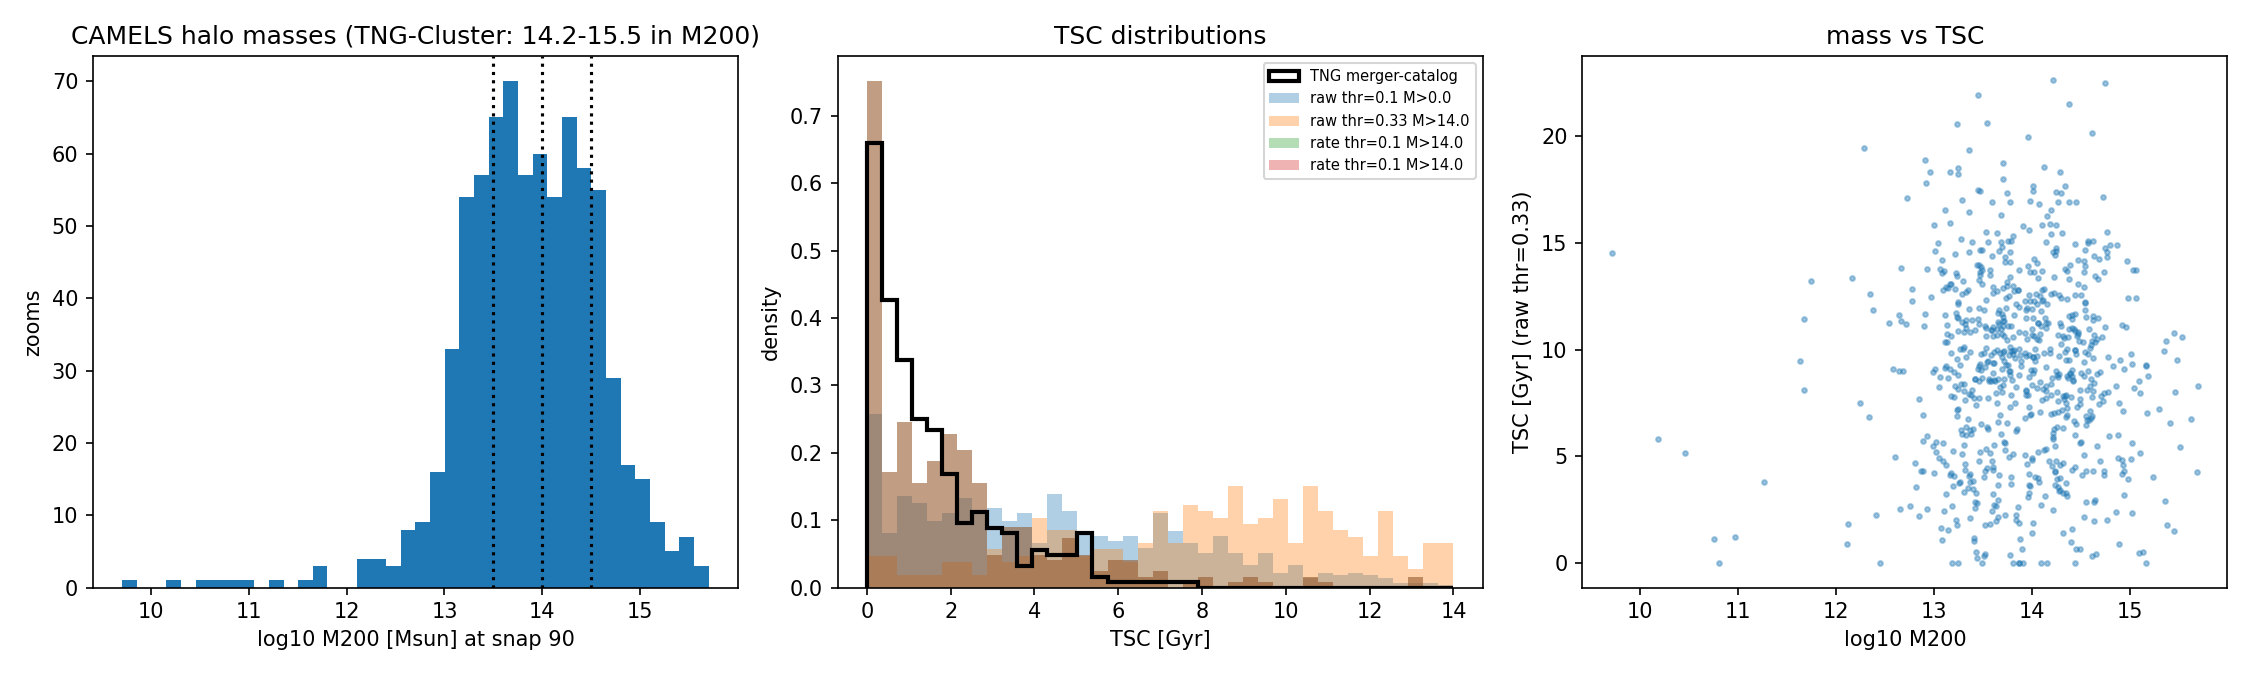
\includegraphics[width=\columnwidth]{camels_mass_tsc.png}
  \caption{CAMELS zooms: mass against the proxy merger time. Adding CAMELS
  to training did not help, because the label, not the images, is the
  bottleneck.}
  \label{fig:camels}
\end{figure}

\bsp
\label{lastpage}
\end{document}
